\subsection{Static matching of the extended configuration interaction}
Adding explicit configuration interaction to density-functional diagonal
energies requires deciding which correlation is already represented.
DFT/MRCI addresses this
issue through an effective Hamiltonian with empirical damping.\cite{marian2019mrci}
We examine zero-frequency self-energy subtraction, following its use in
extended response theories.\cite{tselyaev2013,gambacurta2015}
The borrowed principle is static matching. Its molecular OO-CID application
is a development proposal, rather than an exact density-functional result.

After removing the native ground CSF, define
$\widetilde H=P_g^\dagger(H-E_gS)P_g$ and
$\widetilde S=P_g^\dagger SP_g$. The fixed primary space contains the
optimized singlets and their paired partners; the complementary space
contains all canonical auxiliary configurations. Metric orthogonalization
of the latter gives
\begin{align}
 X&=\widetilde S_{PP}^{-1}\widetilde S_{PQ},\qquad
 A=\widetilde H_{PP},\qquad V=\widetilde H_{PQ}-AX,\\
 D&=\widetilde H_{QQ}-\widetilde H_{QP}X
       -X^\dagger\widetilde H_{PQ}+X^\dagger AX.
\end{align}
Adding $VD^{-1}V^\dagger$ to the primary block in these coordinates yields
\begin{equation}
 H_{\mathrm{eff}}^{\mathrm{sub}}(\omega)
 =A+VD^{-1}V^\dagger+V(\omega S_Q-D)^{-1}V^\dagger,
 \qquad H_{\mathrm{eff}}^{\mathrm{sub}}(0)=A ,
\end{equation}
where $S_Q=\widetilde S_{QQ}-\widetilde S_{QP}X$.
The complete interacting $D$ is used, rather than its diagonal. Its
positivity is checked before inversion. No damping coefficient, constant
excitation shift or orbital-reference adjustment is fitted. The 50/50
weights, $\lambda=0.9$ and previously calibrated $\eta=0.60$ are unchanged.

On the same 26 exposed states, the MAE changes from 0.198 to 0.183 eV.
The $\pi\pi^*$ and $n\pi^*$ MAEs become 0.209 and 0.160 eV. The maximum
individual error increases from 0.446 to 0.478 eV; all errors remain
below 0.5 eV. Table~\ref{tab:staticmatching} and
Figure~\ref{fig:staticmatching} show both the mean improvement and the
cases that become less accurate. All 24 models reproduce these energies
through the public API, with coherent-singlet spin and accepted-restart
checks. These exposed labels do not provide independent transferability
validation.
\begin{table}[!htbp]\centering\small
\caption{Static-matching development candidate on the same corrected native orbitals, geometries and 26 exposed reference labels. No parameter is refitted. All errors are in eV.}
\label{tab:staticmatching}
\begin{tabular}{lrrrrr}\toprule
Family & States & TDA MAE & Before MAE & Matched MAE & Matched max.\\\midrule
All & 26 & 0.789 & 0.198 & 0.183 & 0.478\\
$\pi\pi^*$ & 12 & 1.514 & 0.216 & 0.209 & 0.478\\
$n\pi^*$ & 14 & 0.168 & 0.183 & 0.160 & 0.411\\
\bottomrule\end{tabular}
\end{table}

\begin{figure}[!htbp]\centering
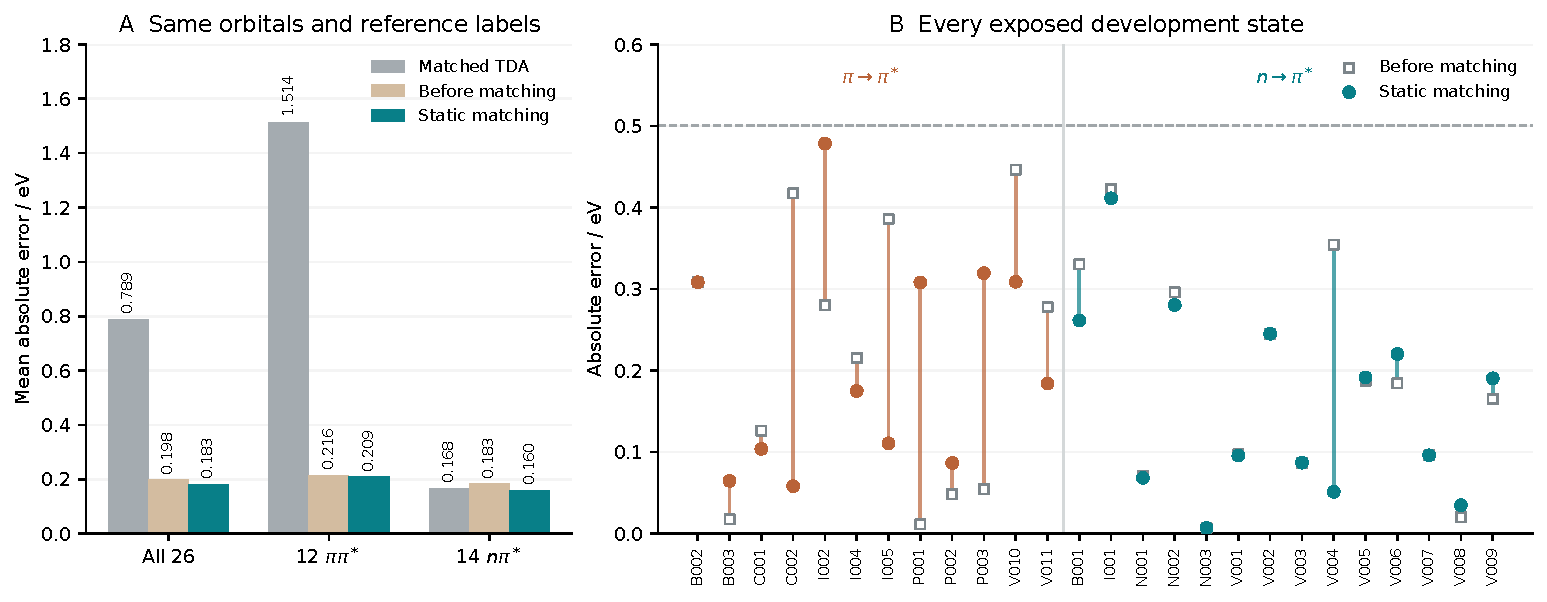
\includegraphics[width=\linewidth]{figures/static_subtraction_accuracy.pdf}
\caption{Static matching on the unchanged exposed development set.
(A) Family-resolved MAEs compared with the unsubtracted candidate and
matched TDA on the same corrected native GFN2 orbitals. (B) Every individual
absolute error before and after matching. The dashed line marks 0.5 eV.
No parameter is refitted and no molecule or state-family branch is added.
This is a development comparison rather than blind validation.}
\label{fig:staticmatching}
\end{figure}

The counterterm participates in the complete analytic nuclear response.
Both derivatives of $D^{-1}$, the metric orthogonalization, the moving
ground projector and $E_g$ are differentiated. Freezing this counterterm
after its vertical evaluation would define a different surface.
The checksummed manifest field
\texttt{static\_self\_energy\_subtraction} selects this candidate through
the existing MOUSE/LINK interface. Older manifests retain their original
Hamiltonian and restart identity. Ethylene's full analytic Hessian takes
9.82 s in a two-thread run. Independent reconverged scalar-energy checks
give maximum directional gradient and curvature errors of
$1.9\times10^{-11}$ Ha/bohr and $3.1\times10^{-8}$ Ha/bohr$^2$.
Furan's complete 27-coordinate Hessian takes 1386.40 s in the serial
column implementation and 297.18 s with eight worker processes (4.67-fold
wall-time reduction). The complete energy, gradient and Hessian arrays
agree exactly between these runs. The serial surface passes independent
scalar-energy checks with maximum gradient and curvature errors of
$1.2\times10^{-10}$ Ha/bohr and $6.6\times10^{-8}$ Ha/bohr$^2$.
Workers reuse the converged orbital states and differentiate the analytic
response columns; no electronic reoptimization is repeated per column.
These timings exclude reference preparation and are not speedup claims
against TDA. Finite differences enter validation only.

The pigment extension tests a different aspect. At the matched
13-orbital frontier, $\beta$-carotene retains a weak lowest state at
2.244 eV ($f=1.58\times10^{-4}$), followed by a dominant absorbing
root at 3.031 eV ($f=5.00$). The bright state is root 4; root 3 at
2.875 eV is weak. This assignment uses recomputed transition moments,
whose unsubtracted replay exactly reproduces the stored convention.
The chlorophyllide lowest gaps at $N=W=16$ become 2.019 and 2.226 eV,
instead of 1.246 and 1.425 eV before matching. These changes are not
a constant shift. The first two roots satisfy the two-increment 0.02 eV
test over $N=14,15,16$ in both matched and fixed-screening sequences.
Higher roots require further frontier and target-coverage checks; a fully
converged static-matched chlorophyllide spectrum is not yet claimed.
Neither pigment enters the 26-state accuracy statistics, and the pigment
adapter does not supply qualified nuclear derivatives.
